%%
% This is an Overleaf template for presentations
% using the TUM Corporate Desing https://www.tum.de/cd
%
% For further details on how to use the template, take a look at our
% GitLab repository and browse through our test documents
% https://gitlab.lrz.de/latex4ei/tum-templates.
%
% The tumbeamer class is based on the beamer class.
% If you need further customization please consult the beamer class guide
% https://ctan.org/pkg/beamer.
% Additional class options are passed down to the base class.
%
% If you encounter any bugs or undesired behaviour, please raise an issue
% in our GitLab repository
% https://gitlab.lrz.de/latex4ei/tum-templates/issues
% and provide a description and minimal working example of your problem.
%%

%\makeatletter
%\def\input@path{{../beamer/}}
%\makeatother

\documentclass[
  german,            % define the document language (english, german)
  aspectratio=169,    % define the aspect ratio (169, 43)
  % handout=2on1,       % create handout with multiple slides (2on1, 4on1)
  % partpage=false,     % insert page at beginning of parts (true, false)
  % sectionpage=true,   % insert page at beginning of sections (true, false)
]{tumbeamer}


% load additional packages
\usepackage{booktabs}
\usepackage{graphicx}
\usepackage{tikz}
\usepackage{url}
\usepackage{pgfplots}
\usepackage{hyperref}
\usepackage{pmboxdraw}
\usepackage{float}
\usepackage{listings}
\usepackage{circuitikz}
%\usepackage[european]{circuitikz}

% image path
\graphicspath{ {./resources/} }

% presentation metadata
\title{Übung 08: Automaten und \\Multi-Cycle-Prozessor}
\subtitle{Einführung in die Rechnerarchitektur}
\author{Niklas Ladurner}

\institute{\theChairName\\\theDepartmentName\\\theUniversityName}
\date[\today]{\today}

\footline{\insertauthor~|~\insertshorttitle~|~\insertshortdate}


% macro to configure the style of the presentation
\TUMbeamersetup{
  title page = TUM tower,         % style of the title page
  part page = TUM toc,            % style of part pages
  section page = TUM toc,         % style of section pages
  content page = TUM more space,  % style of normal content pages
  tower scale = 1.0,              % scaling factor of TUM tower (if used)
  headline = TUM threeliner,      % which variation of headline to use
  footline = TUM default,         % which variation of footline to use
  % configure on which pages headlines and footlines should be printed
  headline on = {title page},
  footline on = {every page, title page=false},
}

% available frame styles for title page, part page, and section page:
% TUM default, TUM tower, TUM centered,
% TUM blue default, TUM blue tower, TUM blue centered,
% TUM shaded default, TUM shaded tower, TUM shaded centered,
% TUM flags
%
% additional frame styles for part page and section page:
% TUM toc
%
% available frame styles for content pages:
% TUM default, TUM more space
%
% available headline options:
% TUM empty, TUM oneliner, TUM twoliner, TUM threeliner, TUM logothreeliner
%
% available footline options:
% TUM empty, TUM default, TUM infoline


\begin{document}

\maketitle

\begin{frame}[c]{}{}
  \begin{center}
    \LARGE  Durchzählen!
  \end{center}
\end{frame}

\begin{frame}[c]{}{}
  \begin{center}
    \LARGE  Keine Garantie für die Richtigkeit der Tutorfolien: Bei Unklarheiten/Unstimmigkeiten
    haben VL/ZÜ-Folien Recht!
  \end{center}
\end{frame}

\begin{frame}[fragile, c]{Endliche Automaten}{}
  \begin{itemize}
    \item Repräsentiert Funktion einer sequentiellen Schaltung (sequentiell: von Zuständen abhängig)
    \item Mathematische Beschreibung als 6-Tupel $(I, O, S, s_0, \delta, \lambda)$
    \item Als Diagramm: Zustände $\rightarrow$ Kreise, Übergänge $\rightarrow$ Verbindungen, Bedingungen $\rightarrow$ Kantenbeschriftungen
    \item One-Hot-Kodierung: Genau 1 FF ist auf 1 $\rightarrow$ aktueller Zustand, einfach aber verschwenderisch
    \item Binärkodierung: FFs zusammen bilden Binärzahl des aktuellen Zustands, spart FFs aber komplexer
  \end{itemize}
  \begin{table}[]
    \begin{tabular}{c|c|c}
    Zustand & One-Hot-Enkodierung & Binärenkodierung \\ \hline
    $S_0$    & $0001$                & $00$               \\
    $S_1$    & $0010$                & $01$               \\
    $S_2$    & $0100$                & $10$               \\
    $S_3$    & $1000$                & $11$              
    \end{tabular}
    \end{table}
\end{frame}

\begin{frame}[fragile, c]{Endliche Automaten}{}
  \begin{center}
    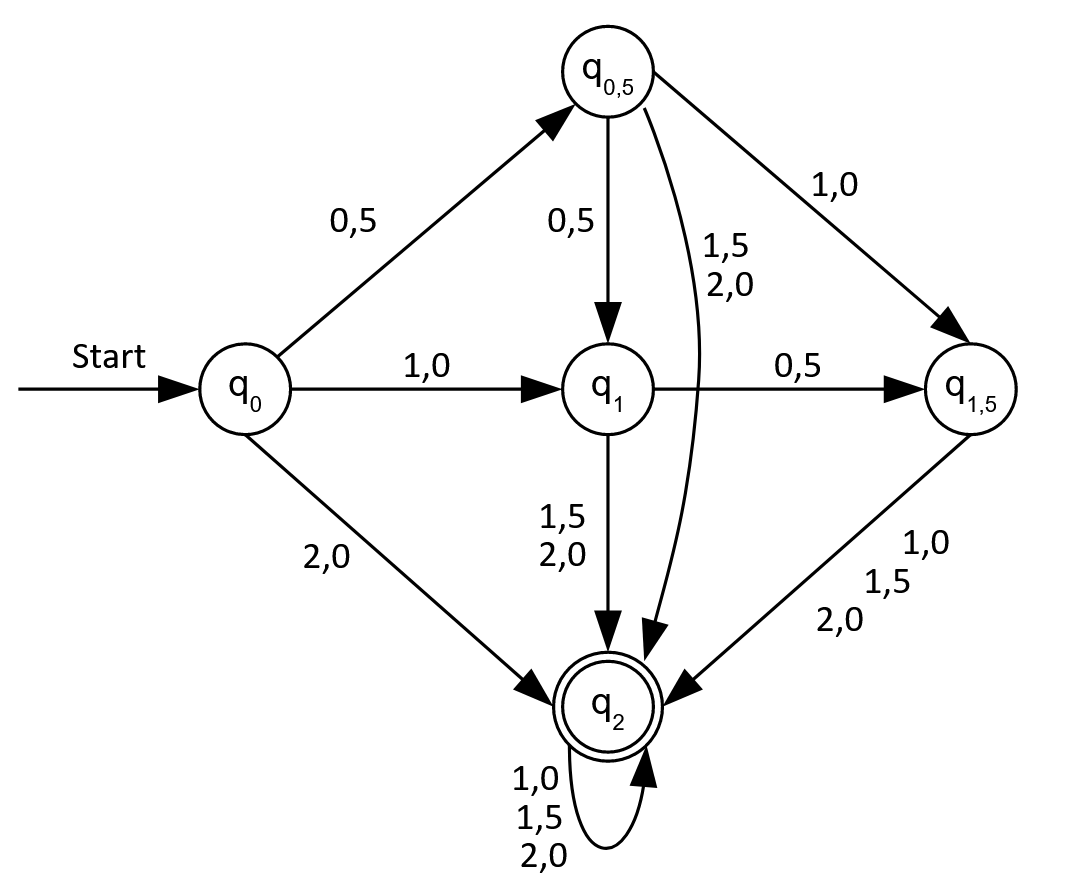
\includegraphics[width=0.6\textwidth]{w08_finite_state_machine.png}
  \end{center}
\end{frame}


\begin{frame}[c, fragile]{RISC-V Multi-Cycle-Prozessor}{}
  \begin{itemize}
    \item Aufteilung einer Instruktion in mehrere Schritte
    \item kürzere kritische Pfade in den einzelnen Teilschritten $\rightarrow$ höhere Taktfrequenz möglich
    \item allerdings benötigt eine Instruktion jetzt auch mehrere Taktzyklen!
    \item komplexeres Steuerwerk, da Zustandsautomat umgesetzt werden muss
    \item (in der Praxis haben sich MC-Prozessoren nicht durchgesetzt)
  \end{itemize}
\end{frame}

\begin{frame}[c]{RISC-V Multi-Cycle-Prozessor}{}
  \begin{center}
    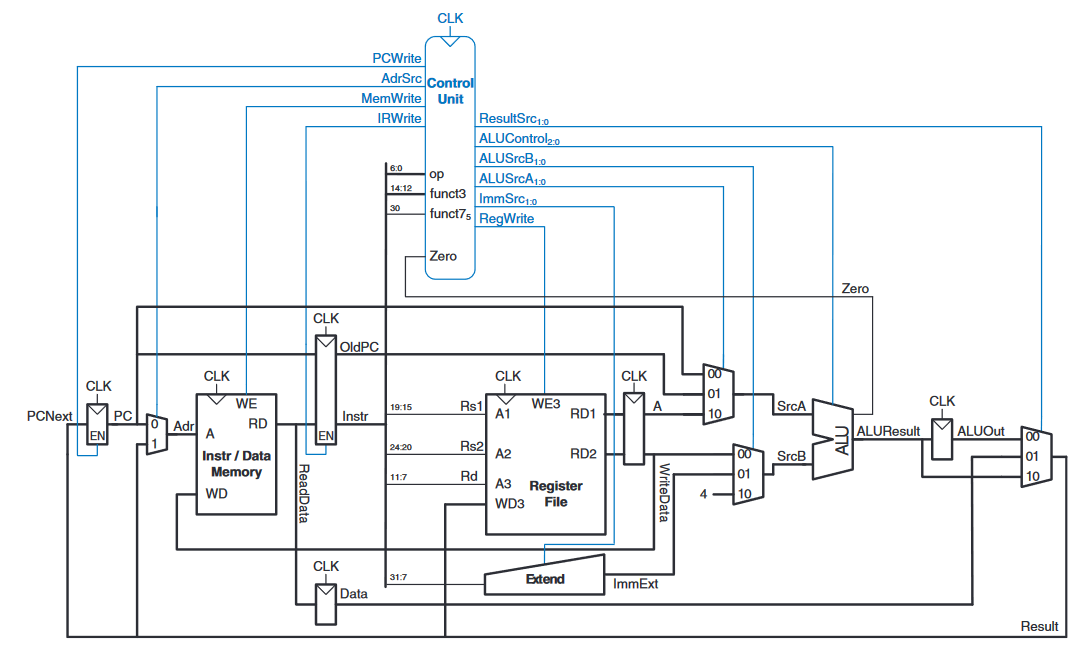
\includegraphics[width=0.75\textwidth]{w08_multi_cycle.png}
  \end{center}
  \centering
  \tiny (Quelle: Vorlesungsmaterialien ERA)
\end{frame}

\begin{frame}[c]{RISC-V Multi-Cycle-Prozessor: Zustandsautomat}{}
  \begin{center}
    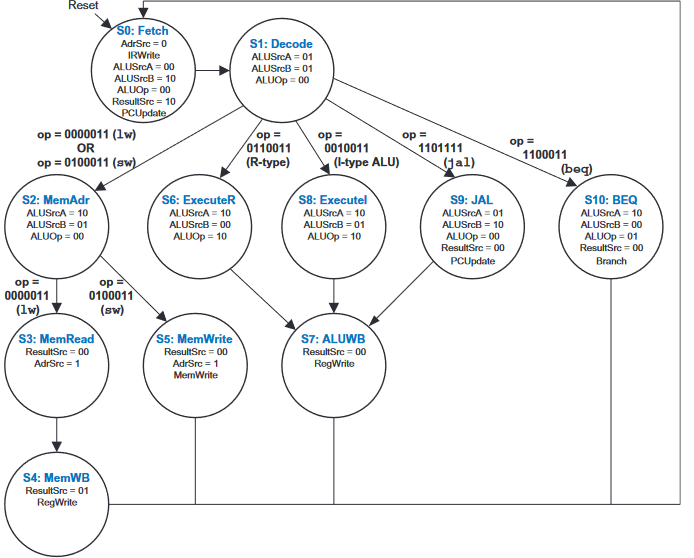
\includegraphics[width=0.6\textwidth]{w08_multi_cycle_states.png}
  \end{center}
  \centering
\end{frame}

\begin{frame}[c]{}{}
  \begin{center}
    \LARGE Fragen?
  \end{center}
\end{frame}

\begin{frame}[c, fragile]{Artemis-Hausaufgaben}{}
  \begin{itemize}
    \item H08 - RISCV Multi bis 17.12.2023 23:59 Uhr
    \item ziemlich aufwendig, aber größtenteils nur Übertragen von Daten aus den Referenztabellen
  \end{itemize}
\end{frame}

\begin{frame}[fragile, c]{Links}{}
  \begin{itemize}
    \item Zulip: \href{https://zulip.in.tum.de/#narrow/stream/1917-ERA-Tutorium---Mi-1600-MI4}{\glqq ERA Tutorium - Mi-1600-MI4\grqq}
          bzw. \href{https://zulip.in.tum.de/#narrow/stream/1940-ERA-Tutorium---Fr-1100-MW2}{\glqq ERA Tutorium - Fr-1100-MW2\grqq}
    \item \href{https://github.com/logisim-evolution/logisim-evolution/releases}{Logisim Evolution}
    \item \href{https://courses.edx.org/assets/courseware/v1/f06a2dc0c856f60ec0711e9f5e1c98cf/asset-v1:HarveyMuddX+ENGR85B+1T2023+type@asset+block/FinalReferences.pdf}{Referenztabellen (offizielle Tabellen sind auf den Übungblättern)}
  \end{itemize}
\end{frame}

\maketitle

\end{document}
